%\documentclass[wcp]{jmlr}

% For citations
%\usepackage{natbib}

% custom commands
%\newcommand{\R}{\mathbb{R}}

%\jmlrvolume{7}
%\jmlryear{2011}
%\jmlrworkshop{Workshop on Unsupervised and Transfer Learning}

%\title[Unsupervised and Transfer Learning Challenge: a Deep Learning Approach]
%{Unsupervised and Transfer Learning Challenge:\\ a Deep Learning Approach}

%\author{\Name{Gr\'egoire Mesnil$^{1,2}$}\Email{mesnilgr@iro.umontreal.ca}\\
%\Name{Yann Dauphin$^1$}\Email{dauphiya@iro.umontreal.ca}\\
%\Name{Xavier Glorot$^1$}\Email{glorotxa@iro.umontreal.ca}\\
%\Name{Salah Rifai$^1$}\Email{rifaisal@iro.umontreal.ca}\\
%\Name{Yoshua Bengio$^1$}\Email{bengioy@iro.umontreal.ca}\\
%\Name{Ian Goodfellow$^1$}\Email{goodfeli@iro.umontreal.ca}\\
%\Name{Erick Lavoie$^1$}\Email{lavoeric@iro.umontreal.ca}\\
%\Name{Xavier Muller$^1$}\Email{mullerx@iro.umontreal.ca}\\
%\Name{Guillaume Desjardins$^1$}\Email{desjagui@iro.umontreal.ca}\\
%\Name{David Warde-Farley$^1$}\Email{wardefar@iro.umontreal.ca}\\
%\Name{Pascal Vincent$^1$}\Email{vincentp@iro.umontreal.ca}\\
%\Name{Aaron Courville$^1$}\Email{courvila@iro.umontreal.ca}\\
%\Name{James Bergstra$^1$}\Email{bergstrj@iro.umontreal.ca}\\
%\addr{$^1$ Dept. IRO, Universit\'e de Montr\'eal. Montr\'eal (QC), H2C 3J7, Canada}\\
%\addr{$^2$ LITIS EA 4108, Universit\'e de Rouen. 76 800 Saint Etienne du Rouvray, France}}
%\addr{$^2$ Dept. LITIS, Universit\'e de Rouen. Mont-Saint-Aignan, 76130, France}}

%\editor{I. Guyon, G. Dror, V. Lemaire, G. Taylor, and D. Silver}

%\begin{document}
%\maketitle

\newcommand{\squeezeup}{\vspace{-2.5mm}}

\iffalse
\begin{abstract}

Learning good representations from a large set of unlabeled data is a
particularly challenging task. Recent work (see \citep{Bengio-2009} for
a review) shows that training deep architectures is a good way to extract such
representations, by extracting and disentangling gradually higher-level 
factors of variation characterizing the input
distribution. In this paper, we describe different kinds of layers we trained
for learning representations in the setting of the Unsupervised 
and Transfer Learning Challenge. The strategy of our
team won the final phase of the challenge. It 
combined and stacked different one-layer unsupervised learning algorithms,
adapted to each of the five datasets of the
competition. This paper describes that strategy and the particular one-layer
learning algorithms feeding a simple linear
classifier with a tiny number of labeled training samples (1 to 64 per class).

\end{abstract}

\begin{keywords}
Deep Learning, Unsupervised Learning, Transfer Learning,
Neural Networks, Restricted Boltzmann Machines, Auto-Encoders,
Denoising Auto-Encoders.
\end{keywords}
\fi
\chapter{Unsupervised and Transfer Learning Challenge: a Deep Learning Approach\label{chap:utlc}}

\section{Introduction}

% Les algos en machine learning sont en général développé dans un tel contexte
% Ici on se place dans le contexte du transfer learning ou les labels pour la tache final
% ne sont pas disponibles mais on a des labels correspondant à d'autres tâches.

The objective of machine learning algorithms is to discover statistical structure
in data. In particular, {\em representation-learning algorithms} attempt to
transform the raw data into a form from which it is easier to perform
supervised learning tasks, such as classification. This is particularly important
when the classifier receiving this representation as input is linear
and when the number of available labeled examples is small. This is the
case here with the Unsupervised and Transfer Learning (UTL) Challenge
\footnote{\tt http://www.causality.inf.ethz.ch/unsupervised-learning.php}.

Another challenging characteristic of this competition is that the training (development) distribution
is typically very different from the test (evaluation) distribution, because it involves
a set of classes different from the test classes, i.e., both inputs and labels
have a different nature. What makes the task feasible is that these different
classes have things in common. The bet we make %with Deep Learning
is that {\em more abstract features of the data are more likely to be shared
among the different classes}, even with classes which are very rare in the
training set. Another bet we make with representation-learning algorithms
and with Deep Learning algorithms in particular is that
the structure of the input distribution $P(X)$
is strongly connected with the structure of the class predictor $P(Y|X)$
for all of the classes $Y$. It means that representations $h(X)$
of inputs $X$ are useful both to characterize $P(X)$ and to characterize
$P(Y|X)$, which we will think of as parametrized through $P(Y|h(X))$.
Another interesting feature of this competition is that the
input features are anonymous, so that teams are compared based on the strength
of their learning algorithms and not based on their ability to engineer
hand-crafted features based on task-specific prior knowledge.
More material on Deep Learning can be found in a companion paper~\citep{Bengio-DL-2011}.

The paper is organized as follows. The pipeline going from bottom (raw data)
to top (final representation fed to the classifier) is described in
\ref{sec:method}.  In addition to the score returned by the competition
servers, \ref{sec:criterion} presents other criteria that guided the
choice of hyperparameters. \ref{sec:results} precisely describes the
layers we chose to combine for each of the five competition datasets, at the end
of the exploration phase that lasted from January 2011 to mid-April 2011.

\section{Method}\label{sec:method}

We obtain a deep representation by
stacking different single-layer blocks, each taken from a small set of possible
learning algorithms, but each with its own set of hyper-parameters (the most
important of which is often just the dimension of the representation).
Whereas the number of possible combinations
of layer types  and hyper-parameters
is exponential as depth increases, we used a greedy layer-wise
approach \citep{Bengio-nips-2006} for building each deep model. Hence, the first
layer is trained on the raw input and its hyper-parameters are chosen with respect to
the score returned by the competition servers (on the validation set) and different criteria
to avoid overfitting to a particular subset of classes 
(discussed in \ref{sec:criterion}). We then fix the 
$i^{th}$ layer (or keep only a very small number of choices)
and search for a good choice of the $i+1^{th}$ layer, pruning
and keeping only a few good choices.
Depth is thus increased without an explosion in computation
until the model does not improve significantly the performance
according to our criteria.

The resulting learnt pipeline can be divided in three types
of stages: preprocessing, feature
extraction and transductive postprocessing.

\subsection{Preprocessing}\label{sec:preproc}
% Grégoire, Xavier


Before the feature extraction step, we preprocessed the data using various
techniques. Let $\mathcal{D}=\{ x^{(j)} \}_{j=1,\dots, n}$ be a training set
where $x^{(j)}\in\mathbb{R}^d$.

\paragraph{Standardization} One option is to standardize the data. For each
feature, we compute its mean $\mu_k=(1/n)\sum_{j=1}^n x^{(j)}_k$ and variance
$\sigma_k$. Then, each transformed feature $\tilde{x}^{(j)}_k=(x^{(j)}_k -
\mu_k )/ \sigma_k$ has zero mean and unit variance.

\paragraph{Uniformization (t-IDF)} Another way to control the range of the
input is to uniformize the feature values by restricting their possible values
to $[0,1]$ (and non-parametrically and approximately mapping each feature to a
uniform distribution). We rank all the $x^{(j)}_k$ and  map them to $[0,1]$ by
dividing the rank by the number of observations sorted. In the case of sparse data,
we assigned the same range value (0) for zeros features. One option is
to aggregate all the features in these statistics and another is to do it
separately for each feature.

\paragraph{Contrast Normalization} On datasets which are supposed to correspond
to images, each input $d$-vector is normalized with respect to the values
in the given input vector (global contrast normalization). For
each sample vector $x^{(j)}$ subtract its mean $\mu^{(j)}=(1/d)\sum_{k=1}^d
x^{(j)}_k$ and divide by its standard deviation $\sigma^{(j)}$ (also across the
elements of the vector).  In the case of images, this would discard the
average illumination and contrast (scale).

\paragraph{Whitened PCA} The Karhulen-Lo\`{e}ve transform constantly improved the
quality of the representation for each dataset. Assume the training set
$\mathcal{D}$ is stored as a matrix $X\in\mathcal{M}_\mathbb{R}(n,d)$. First,
we compute the empirical mean $\mu=(1/n)\sum_{i=1}^n X_{i.}$ where $X_{i.}$
denotes row $i$ of the matrix $X$, i.e., example $i$. 
We center the data $\tilde{X}=X-\mu$ and
compute the covariance matrix $C=(1/n)\tilde{X}^T\tilde{X}$.  Then, we obtain the
eigen-decomposition of the covariance matrix $C=V^{-1}UV$ i.e
$U\in\mathbb{R}^d$ contains the eigen-values and
$V\in\mathcal{M}_{\mathbb{R}}(d,d)$ the corresponding eigen-vectors (each row
corresponds to an eigen-vector).  We build a diagonal matrix $U^{'}$ where
$U^{'}_{ii}=\sqrt{C_{ii}}$.  By the end, the output of the whitened PCA is
given by $Y=(X-\mu)VU^{'}$. In our experiments, we used the PCA 
implementation of the scikits
\footnote{http://scikits.appspot.com/} toolbox. 


\paragraph{Feature selection} In the datasets where the input is sparse, a
preprocessing that we found very useful is the following: {\em only the
features active on the training (development) {\bf and} test (resp. validation)
datasets are retained} for the test set (resp. validation) representations.  We
removed those whose frequency was low on both datasets (this introduces a new
hyper-parameter that is the cut-off threshold, but we only tried a couple of
values).

\subsection{Feature extraction}

Feature extraction is the core of our pipeline and has been crucial for getting
the first ranks during the challenge. Here we briefly introduce each method
that has been used during the competition. See also \citep{Bengio-DL-2011}
along with the citations below for more details.

\subsubsection{$\mu$-ss-RBM}
%Guillaume, Aaron

The $\mu$-spike and slab Restricted Boltzmann Machine ($\mu$-ssRBM)
\citep{Courville+al-2011} is a recently introduced undirected graphical model
that has demonstrated some promise as a model of natural images. The model
is characterized by having both a real-valued \emph{slab} vector and a
binary \emph{spike} variable associated with each hidden unit. The model
possesses some practical properties such as being amenable to block Gibbs
sampling as well as being capable of generating similar latent
representations of the data to the mean and covariance
Restricted Boltzmann Machine \citep{Ranzato2010b}.

The $\mu$-ssRBM describes the interaction between three random vectors: the
visible vector $v$ representing the observed data, the binary ``spike''
variables $h$ and the real-valued ``slab'' variables $s$.
%
Suppose there are $N$ hidden units and a
visible vector of dimension $D$: $v\in\mathbb{R}^{D}$.
%
The $i$th hidden unit ($1
\leq i \leq N$) is
associated with a binary \emph{spike} variable: $h_i \in \{0,1\}$ and a real
valued vector $s_i \in \mathbb{R}^{K}$, pooling over $K$ linear
filters. This kind of pooling structure allows the model to \emph{learn}
over which filters the model will pool -- a useful property in the context
of the UTL challenge where we cannot assume a standard ``pixel structure'' in the input.
%
The $\mu$-ssRBM
model is defined via the energy function
{\small
\begin{align}
E(v,s,h) &= -\sum_{i=1}^{N}v^{T}W_{i}s_{i}h_{i} +\frac{1}{2}v^{T}\left(\Lambda+\sum_{i=1}^{N}\Phi_{i}h_{i}\right)v \nonumber \\
         &  +\sum_{i=1}^{N} \frac{1}{2}s_{i}^{T}\alpha_{i}s_{i}\ -\sum_{i=1}^{N} \mu_{i}^{T}\alpha_{i}s_{i}h_{i}
            -\sum_{i=1}^{N}b_{i}h_{i} +\sum_{i=1}^{N}\mu_{i}^{T}\alpha_{i}\mu_{i}h_{i}, \nonumber
\label{eq:mu_energy}
\end{align}
}
in which $W_{i}$ refers to the $i$th weight matrix of size $D\times K$, the
$b_i$ are the biases associated with each of the spike variables $h_i$, and
$\alpha_i$ and $\Lambda$ are diagonal matrices that penalize large values
of $\Vert s_i \Vert_2^2$ and $\Vert v \Vert_2^2$ respectively. 

\bigskip

Efficient learning and inference in the $\mu$-ssRBM is rooted in the ability to
iteratively sample from the factorial conditionals $P(h \mid v)$, $p(s \mid
v,h)$ and $p(v \mid s, h)$ with a Gibbs sampling procedure. For a detailed
derivation of these conditionals, we refer the reader to \citep{Courville+al-2011}.
In training the $\mu$-ssRBM, we use stochastic maximum likelihood
~\citep{Tieleman08} to update the model parameters.


\subsubsection{Denoising Autoencoder}
% Pascal V
Traditional autoencoders map an input $x \in \R^{d_x}$ to a hidden
representation $h$ (the learnt features) with an affine mapping followed by a non-linearity $s$
(typically a sigmoid): $h = f(x) = s(Wx+b)$. The representation is then mapped back to
input space, initially producing a linear reconstruction $r(x)=W'f(x)+b_r$, where $W'$ can
be the transpose of $W$ (tied weights) or a different matrix (untied
weights).  The autoencoder's parameters $\theta={W,b,b_r}$ are optimized so
that the reconstruction is close to the original input $x$ in the sense of
a given loss function $L(r(x),x)$ (the reconstruction error). 
Common loss functions include squared error
$\|r(x)-x\|^2$, squared error after sigmoid $\|s(r(x))-x\|^2$, and sigmoid
cross-entropy $-\sum_i x_i \log s(r_i(x)) + (1-x_i) \log(1-s(r_i(x)))$.
To encourage robustness of the representation, and avoid trivial useless
solutions, a simple and efficient
variant was proposed in the form of the Denoising
Autoencoders~\citep{VincentPLarochelleH2008,Vincent-JMLR-2010}. 
Instead of being trained to merely reconstruct its inputs, a Denoising
Autoencoder is trained to \emph{denoise} artificially corrupted training samples, 
a much more difficult task, which was shown to force it to extract more
useful and meaningful features and capture the structure of the
input distribution~\citep{Vincent-JMLR-2010}. In practice, 
instead of presenting the encoder with a clean training sample $x$, it is given
as input a stochastically corrupted version $\tilde{x}$. The objective
remains to minimize reconstruction error $L(r(\tilde{x}),x)$ with respect to clean sample
$x$, so that the hidden representation has to help denoise.  
Common choices for the corruption include additive Gaussian noise, and
masking a fraction of the input components at random by setting them to 0
(masking noise).

\subsubsection{Contractive Autoencoder}
% Grégoire
% copy/paste re-write it
To encourage robustness of the representation $f(x)$ obtained for a training
input $x$, \citep{Rifai+al-2011} propose to penalize its {\em sensitivity} to
that input, measured as the Frobenius norm of the Jacobian $J_f(x)$
of the non-linear mapping. Formally, if input $x \in \R^{d_x}$ is mapped by an encoding
function $f$ to a hidden representation $h \in \R^{d_h}$, this sensitivity
penalization term is the sum of squares of all partial derivatives of the
extracted features with respect to input dimensions: \begin{equation}
\nonumber\|J_f(x)\|_F^2 = \sum_{ij} \left( \frac{\partial h_j(x)}{\partial x_i}
\right)^2.  \label{eq:sensitivity} \end{equation}

Penalizing $\|J_f\|_F^2$ encourages the mapping to the feature space to be
contractive in the neighborhood of the training data.   The {\em flatness}
induced by having small first derivatives will imply an {\em invariance}
or {\em robustness} of the representation for small variations of the input.

While such a Jacobian term alone would encourage mapping to a useless constant
representation, it is counterbalanced in auto-encoder training by the need for
the learnt representation to allow a good reconstruction of the training
examples.


\subsubsection{Rectifiers}
% Xavier

%In the context of neural networks, the choice of the activation function is an
%important subject. The most commonly used activation function is the
%\emph{logistic sigmoid}, inspired from the ``S'' shaped firing rate response of
%biological neurons. However, from the optimization standpoint the non-zero
%steady state of this non-linearity has been shown to hurt gradient-based
%optimization~\citep{LeCun+98backprop,GlorotAISTATS2010}.  The \emph{hyperbolic
%tangent}, which has its steady state at $0$, is therefore preferred. 


Recent works investigated linear rectified activation function variants.
\citep{Nair+Hinton-2010} used Noisy Rectified Linear Units (NReLU) (i.e.
$\max(0,x+N(0,\sigma(x))$) for Restricted Boltzmann Machines.  Compared to
binary units, they observed significant improvements in term of generalization
performance for image classification tasks. Following this line of work,
\citep{Glorot+al-AI-2011} used the rectifier activation function (i.e.
$\max(0,x)$) for deep neural networks and Stacked Denoising Auto-Encoders
(SDAE)~\citep{VincentPLarochelleH2008,Vincent-JMLR-2010} and obtained 
similarly good results.


This non-linearity has various mathematical advantages. First, it naturally 
creates sparse representations with true zeros which are computationally 
appealing. In addition, the linearity on the active side of the activation function
allows gradient to flow well on the active set of neurons, possibly reducing the 
vanishing gradients problem.

In a semi-supervised setting similar to that of the Unsupervised and
Transfer learning Challenge setup, \citep{Glorot+al-AI-2011} obtained 
state-of-the-art results for a sentiment analysis task (the Amazon 4-task benchmark) 
for which the  bag-of-words input were highly sparse.
% Already in the results section
%Therefore, we chose to
%use the same model: a DAE with rectifier units, for the datasets {\bf HARRY} and {\bf TERRY}.  

% Yann
But learning such embeddings for huge sparse vectors with the proposed approach
is still very expensive. Even though the training cost only scales linearly
with the dimension of the input, it can become too expensive when the input
becomes very large. Projecting the input vector to its embedding can be made
quite efficient by using a sparse matrix-vector product. However, projecting
the embedding back to the input space is quite expensive during decoding because
one has to compute a reconstruction (and reconstruction error)
for all inputs and not just the non-zeros. If
the input dimension is 50,000 and the embedding dimension 1,000 then decoding
requires 50,000,000 operations. In order to speed-up training for huge sparse
input distributions, we use reconstruction sampling \citep{Dauphin+al-2011}. The
idea is to reconstruct all the non-zero elements of the input and a small
random subset of the zero elements, and to use importance sampling weights
to exactly correct the bias thus introduced.

The learning objective is sampled in the following manner: \[ \hat{L}({\bf x},
{\bf z}) = \sum_k^d \frac{\hat{\bf p}_k}{{\bf q}_k} H({\bf x}_k, {\bf z}_k) \]
where $\hat{\bf p} \in \{0, 1\}^{d_x}$ with $\hat{\bf p} \sim P(\hat{\bf
p}|{\bf x})$. The sampling pattern $\hat{\bf p}$ is resampled for each
presentation of the input and it controls which input unit will participate in
the training cost for this presentation. The bias introduced by sampling can be
corrected by setting the reweighting term $1/{\bf q}$ such that ${\bf
q}_k=E[\hat{\bf p}_k|k,{\bf x},\tilde{\bf x}]$.

The optimal sampling probabilities $P(\hat{\bf p}|{\bf x})$ are those that
minimize the variance of the estimator $\hat{L}$. \citep{Dauphin+al-2011} show that
reconstructing all non-zeros and a small subset of zeros is a good heuristic.
The intuition is that the model is more likely to be wrong on the non-zeros
than the zeros. Let ${\cal C}({\bf x},\tilde{\bf x})=\{k: {\bf x}_k=1 \;{\rm
or}\;\tilde{\bf x}_k=1\}$. Then bit $k$ is reconstructed with probability
\begin{equation} \label{eq:p} P(\hat{\bf p}_k=1|{\bf x}_k) = \left\{
    \begin{array}{ll} 1 & {\rm if}\; k \in {\cal C}({\bf x},\tilde{\bf x}) \\
    |{\cal C}({\bf x},\tilde{\bf x})|/d_x & otherwise \end{array} \right.
\end{equation}

\citep{Dauphin+al-2011} show that the computational speed-up is on the order of
$^{d_{SMP}}/_{d_x}$ where $d_{SMP}$ is the average number of units that are
reconstructed and $d_x$ is the input dimension. Furthermore, reconstruction sampling
yields models that converge as fast as the non-sampled networks in terms of gradient steps
(but where each step is much faster).


\subsection{Postprocessing}
% Ian

The competition servers use a Hebbian classifier. Specifically,
the discriminant function applied to a test set matrix 
$Z$ (one row per example) after training
the representation on a training set matrix $X$ (one row per example) is given by
\[ f(Z) = Z X^T y \]
where $y_i = 1 / n_p$ if training example $i$ is positive,
or $-1/n_n$ if training example $i$ is negative, where $n_p$ and $n_n$
are the number of positive and negative training examples, respectively.
One classifier per class (one against all) is trained.

This classifier does not have any regularization hyperparameters.
We were interested in discovering whether some postprocessing of our
features could result in Hebbian learning behaving as if it was regularized.
It turns out that in a sense, Hebbian learning is already maximally
regularized. Fisher discriminant analysis can be solved as a linear
regression problem~\citep{bishop-book2006}, and the L2 regularized version
of this problem yields this discriminant function:
\[ g_\lambda(Z) = Z (X^T X + \lambda I) X^T y \]
where $\lambda$ is the regularization coefficient. Note that
\[ \lim_{\lambda\rightarrow\infty} \frac{g_\lambda(Z)}{||g_\lambda(Z)||} = \frac{f(Z)}{||f(Z)||}. \]
Since scaling does not affect the final classification
decision, Hebbian learning may be seen as maximally regularized Fisher
discriminant analysis. It is possible to reduce Hebbian learning's implicit
L2 regularization coefficient 
to some smaller $\lambda$ by multiplying $Z$ by $(X^TX+\lambda I)^{-1/2}$),
but it is not possible to increase it.

Despite this implicit regularization, overfitting is still an important
obstacle to good performance in this competition
due to the small number of training examples used. We therefore explored
other means of avoiding overfitting, such as reducing the number of features
and exploring sparse codes that would result in most of the features
appearing in the training set being 0. However, the best results
and regularization were obtained by a transductive PCA.

\subsubsection{Transductive PCA}
% Grégoire

A Transductive PCA is a PCA transform trained not on the training set but on
the test (or validation) set. After training the first $k$ layers of the
pipeline on the training set, we trained a PCA on top of layer $k$, either on
the validation set or on the test set (depending on whether we were submitting
to the validation set or the test set). Regarding the notation used in
~\ref{sec:preproc}, we apply the same transformation with $X$ replaced by the
representation on top of layer $k$ of the validation set or the test set i.e
$h(X_{valid})$.

This transductive PCA thus only retains variations that are the dominant ones
in the test or validation set. It makes sure that the final classifier will
ignore the variations present in the training set but irrelevant for the test
(or validation) set.  In a sense, this is a generalization of the strategy
introduced in ~\ref{sec:preproc} of removing features that were not present in
the both training and test / validation sets. The lower layers only keep the
directions of variation that are dominant in the training set, while the top
transductive PCA only keeps those that are significantly present in the
validation (or test) set.

We assumed that the validation and test sets contained the same number of classes to
validate the number of components on the validation set performance. In general,
one needs at least $k-1$ components in order to separate $k$ classes by
a set of one-against-all classifiers.
Transductive PCA has been decisive for winning the competition as it improved considerably
the performance on all the datasets. 
In some cases, we also used a mixed strategy for the intermediate layers, mixing
examples from all three sets.

\subsubsection{Other methods}
 

% As we need to fit in 8 pages and we do not actually used t-sne
% we can skip it
%\subsubsection{t-SNE}
% David
%Advertising for cs.toronto
%\subsubsection{Gaussian Mixture Model}

%After we obtained a low-dimensional representation based on denoising autoencoders which was
%performing well, we were able to visualize the data as a three-dimensional scatter 
%plot of the representation learnt. On some datasets, a very clear clustering pattern became
%visually apparent, though it appeared that several clouds came together in
%an ambiguous region of the latent space discovered, in a kind of flower shape
%that we have previously observed in many manifold-learning algorithms. We hypothesize
%that this shape arises because some of the inputs contain less information
%(e.g. less non-zero entries, in the case of sparse high-dimensional textual data)
%which make their class ambiguous. It is natural that in a high-dimensional space,
%ambiguous patterns conglomerate in the ``middle'' while clearer patterns stand
%farther away from the other class clouds.

After the feature extraction process, we were able to visualize the data as a
three-dimensional scatter plot of the representation learnt. On some datasets,
a very clear clustering pattern became visually apparent, though it appeared
that several clouds came together in an ambiguous region of the latent space
discovered.

In order to attempt to disambiguate this ambiguous region without
making hard-threshold decisions, we fit a Gaussian mixture model with the EM
algorithm and a small number of Gaussian components chosen by visual inspection
of these clouds.  We then used the posterior probabilities of the cluster
assignments as an alternate encoding. 

K-means, by contrast with Gaussian mixture models, makes a hard decision as
to cluster assignments. Many researchers were recently impressed when they found out
that a certain kind of feature representation (the ``triangle code'') based on
K-means, combined with specialized pre-processing, yielded state of the art
performance on the CIFAR-10 image classification benchmark~\citep{Coates2011}.
Therefore, we tried K-means with a large number of means and the triangle code as
a post-processing step.

%, which slightly improved our performance on TERRY.
In the end, though, none of our selected final entries included a Gaussian mixture model or K-means,
as the transductive PCA always worked better as a post-processing layer.


%\subsubsection{K-means}
% David

%K-means, by contrast with Gaussian mixture models, makes a hard decision as
%to cluster assignments. While being a well-worn and trusty addition to the
%machine learner's toolbox, its simplicity may lead some to unjustly
%dismiss it. Many researchers were recently impressed when they found out
%that a certain kind of feature representation (the ``triangle code'') based on
%K-means, combined with specialized pre-processing, yielded state of the art
%performance on the CIFAR-10 image classification benchmark~\citep{Coates2011}.
%We tried K-means with a large number of means and the triangle code as
%a post-processing step for several of the tasks, but in the end did not
%select it either for our final entries.

%(Did this improve anything? Ian says no)
% It does not but we can say we tried it --Grégoire

\section{Criterion}\label{sec:criterion}
%In our greedy layer wise strategy for choosing blocks and hyper-parameters
%we tried several criteria, none of them worked but we could say that
%we think about it (and we were not stupid enough to click n'submit 7000 times...).
% Erick
%ALC validation vs test\\
%mean and deviation on several splits

The usual kind of overfitting is due to specializing to particular labeled
examples. In this transfer learning context, another kind of overfitting arose:
overfitting a representation to particular {\em classes}. Since the validation
set and test set have non-intersecting sets of classes, finding representations
that work well on the validation set was not a guarantee for good behavior
on the test set, as we learned from our experience with the competition first phase.
Note also that the competition was focused on a particular criterion,
the Area under the Learning Curve
(ALC)\footnote{http://www.causality.inf.ethz.ch/ul\_data/DatasetsUTLChallenge.pdf}
which gives much weight to the cases with very few labeled examples (1, 2, or 4,
per class, in particular, get almost half of the weight). So the question we
investigated in the second and final phase (where some training set labels
were revealed) was the following: does the ALC of a representation computed
on a particular subset of classes correlate with the ALC of the same
representation computed on a different set of classes?

Overfitting on a specific subset of classes can be observed by training a PCA
separately on the training, validation and test sets on {\bf ULE} (this data
set corresponds to MNIST digits). The number of components maximizing the ALC
will be different, depending on the choice of the subset of classes.
Figure~\ref{fig:alc-overfitting} illustrates the effect of the number of
components retained on the training, validation and test ALCs.  While the best
number of components on the validation set would be 2, choosing this number of
components for the test set significantly degrades the test ALC. 

During the first phase, we noticed the absence of correlation between the validation
ALC and test ALC computed on the {\bf ULE} dataset. During the second phase, we tried
to reproduce the competition setting using the labels available for transfer
with the hope of finding a criteria that would guarantee generalization. The
ALC was computed on every subset of at least two classes found in the transfer
labels and metrics were derived. Those metrics are illustrated in Figure
\ref{fig:alc-criterion}. We observed that the standard deviation seems to be
inversely proportional to the generalization accuracy, therefore substracting it from
the mean ALC ensures that the choice of hyper-parameters is done in a range where
the training, validation and test ALCs are correlated. In the case of a PCA, optimizing
the $\mu - \sigma$ criteria correctly returns the best number of PCA
components, ten, where the training, validation and test ALCs are all correlated.

It appears that this criterion is a simple way to use the small amount of
labels given to the competitors for the phase $2$. However, this criterion has
not been heavily tested during the competition since we always selected our
best models with respect to the validation ALC returned by the competition
servers. From the phase $1$ to the phase $2$, we only explored the space of the
hyperparameters of our models using a finer grid.

\begin{figure}
\centering
\begin{subfigure}{.45\textwidth}
\centering
\includegraphics[height=0.25\textheight,keepaspectratio]{article1/images/alc-overfitting.png}
\caption{ALC on the three sets}
\label{fig:alc-overfitting}
\end{subfigure}
\begin{subfigure}{.45\textwidth}
\centering
\includegraphics[height=0.25\textheight,keepaspectratio]{article1/images/alc-criterion.png}
\caption{Criterion}
\label{fig:alc-criterion}
\end{subfigure}
\caption[ALC Comparison]{
{\bf ULE Dataset} Left: ALC on training, validation and
test sets of PCA representations, with respect to the number of principal components retained.
Right: Comparison between training, validation and test ALC and the criterion computed from
the ALC, obtained on every subset of at least 2 classes present in the transfer
labels for different numbers of components of a PCA.}
\label{fig:alc-comparison}
\end{figure}



\iffalse
\begin{figure*}[h] \centering \subfigure[ALC on the three sets]{\includegraphics[width=0.45\linewidth]{images/alc-overfitting.png}
\label{fig:alc-overfitting}}
\subfigure[Criterion]{\includegraphics[width=0.45\linewidth]{images/alc-criterion.png}
\label{fig:alc-criterion}} 
\caption{
}
\label{fig:alc-comparision}

\end{figure*}
\fi


\section{Results}\label{sec:results}

For each of the five datasets, {\bf AVICENNA}, {\bf HARRY}, {\bf TERRY}, {\bf
SYLVESTER} and {\bf RITA}, the strategy retained for the final winning
submission on the phase 2 is precisely described. Training such a deep stack of
layers from preprocessing to postprocessing takes at most $12$ hours for each
dataset once you have found the good hyperparameters. All our models are
implemented in Theano \citep{bergstra+al:2010-scipy}, a Python library that allows transparent use of GPUs.
During the competition, we used a cluster of GPUs, Nvidia GeForce GTX 580.

\begin{figure}[t]
  \begin{center}
    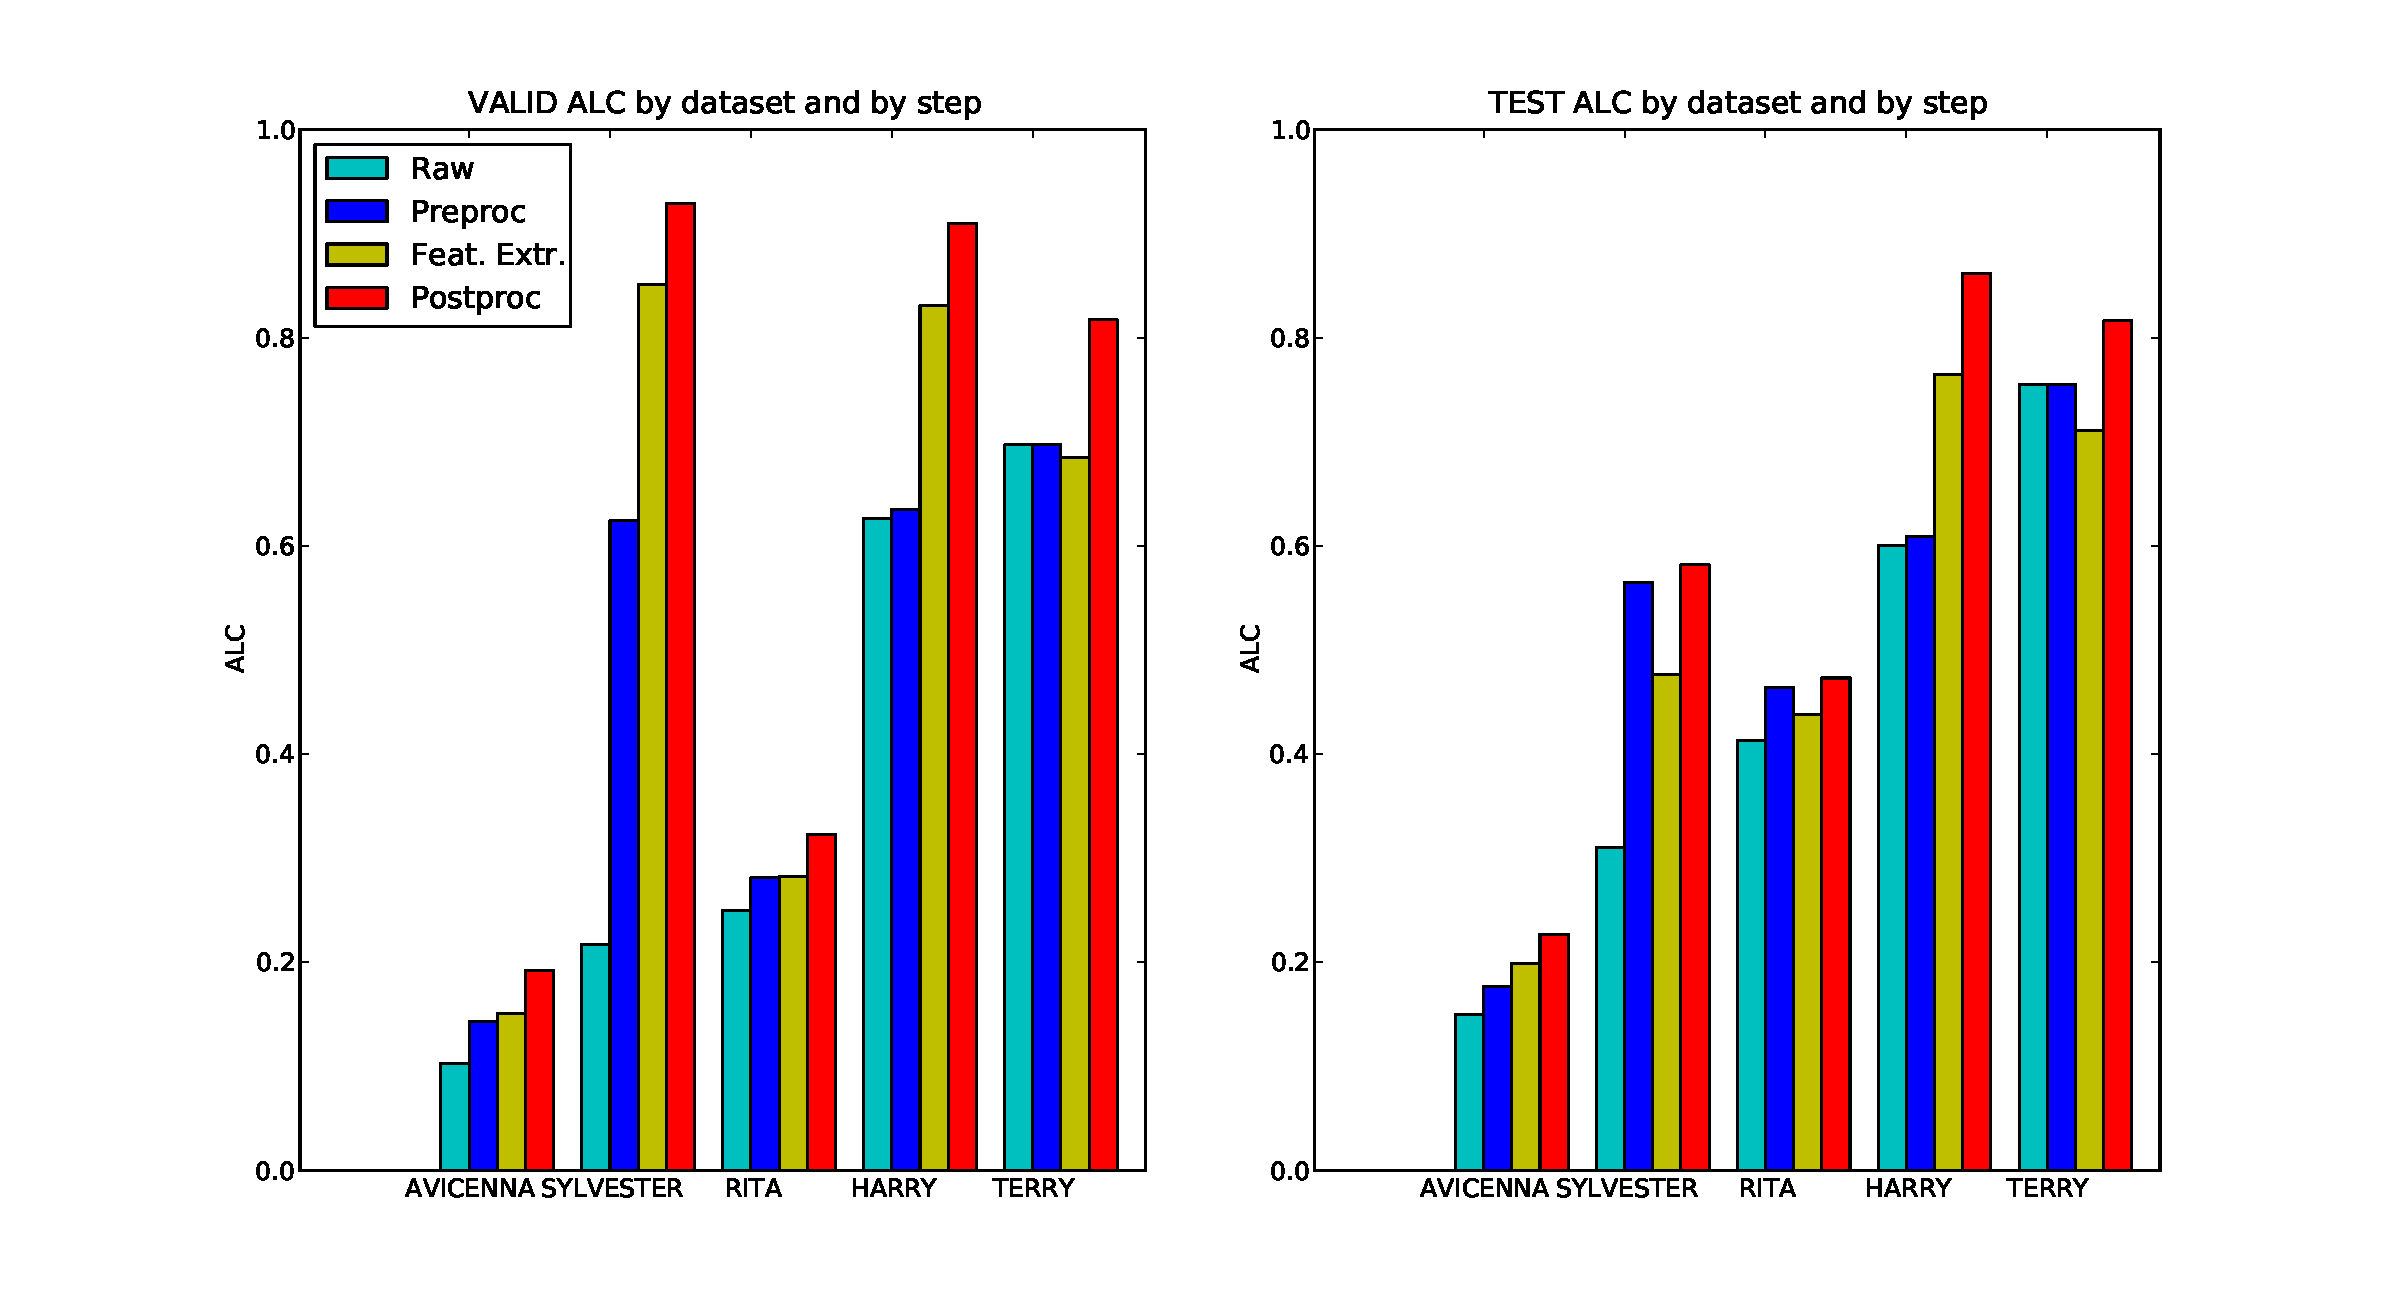
\includegraphics[width=1.\linewidth]{article1/images/5steps.pdf}
    \caption[ALC after each layer on Valid and Test]{\label{fig:charts} For each data set, we report the Validation and Test ALC after each layer (from raw data to postprocessing). It allows us to see where overfitting arose ({\bf SYLVESTER}) and which of the layers resulted the more important to improve the overall performance.}
    \vspace{-0.2in}
  \end{center}
 \vspace*{-1mm}
\end{figure}


 
\subsection{AVICENNA}
% Gregoire preproc pca whitened 75 comp DAE binomial 0.3 noise nhidden 600
% transductive pca  7

\paragraph{Nature of the data}
It corresponds to arabic manuscripts and consists of $150,205$ training samples of dimension $120$.

\paragraph{Best Architecture}
For preprocessing, we fitted a whitened-PCA on the raw data and kept the first
$75$ components in order to eliminate the noise from the input distribution.
Then, the second layer consisted in a Denoising Autoencoder of $600$ hidden
units trained with a binomial noise, i.e, each component of the input had a
probability $p=0.3$ of being masked (set to 0). The top layer was a transductive PCA 
with only the $7$ principal components.

\paragraph{Results}
This strategy ranked first with a validation and final ALC score of $0.1932$
and $0.2273$ respectively. Training a contractive auto-encoder gives similar
results on the validation set i.e a validation and final ALC score of $0.1930$
and $0.1973$ respectively.
% EL: For the next 3 experiments, I kept the personal tone ('we ...').  I can
% rewrite it to a neutral tone if it is not appropriate.  Also, the present
% tense is used.  The fourth experiment use the past tense.  I can rewrite
% those three to past tense to make it more uniform.
\subsection{HARRY}



\paragraph{Nature of the data} It corresponds to human actions and consists of
$69,652$ training samples of dimension $5,000$, which are
sparse: only $~2\%$ of the components
are typically non-zero.

\paragraph{Best Architecture} For the first layer, we uniformized the non-zero
feature values (aggregating all features)
across the concatenation of the training, validation and test
sets.  For the second layer, we trained on the union of the 3 sets a Denoising
Auto-Encoder with rectifier units and reconstruction sampling. We used the
binomial masking noise $(p=0.5)$ as corruption process, the logistic sigmoid as
reconstruction activation function and the cross entropy as reconstruction
error criterion.  The size of the hidden layer was $5000$ 
% as the input
and we added an $L_1$ penalty on the activation values to encourage sparsity of
the representation. For the third layer, we applied a transductive PCA and kept
$3$ components.

\paragraph{Results} We obtained the best validation ALC score of the
competition.  This was also the case for the final evaluation score with an ALC
score of 0.861933, whereas the second best obtained 0.754497.
Figure~\ref{fig:harry} shows the final data representation we obtained for the
test (evaluation) set. 
%     after the transductive PCA.

\begin{figure}[t]
  \begin{center}
    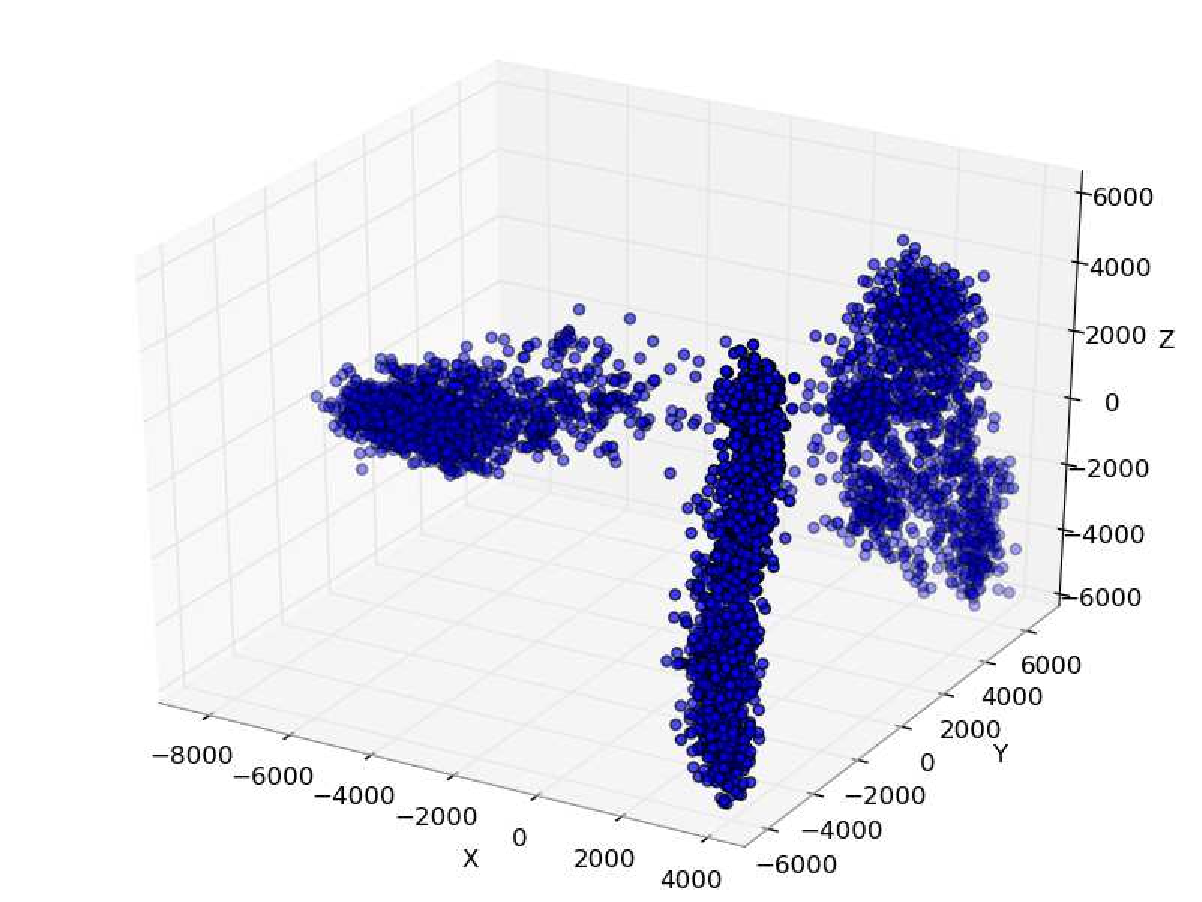
\includegraphics[width=0.75\linewidth]{article1/images/harry_cluster.pdf}
    \caption[Clustering 3D on HARRY]{\label{fig:harry}  {\bf HARRY} evaluation set 
     after the transductive PCA, the data is nicely clustered, suggesting
     that the learned preprocessing has discovered the underlying class structure.}
    \vspace{-0.2in}
  \end{center}
 \vspace*{-1mm}
\end{figure}


\subsection{TERRY}
% Xavier


\paragraph{Nature of the data} This is a natural language processing
(NLP) task, with $217,034$ training samples of dimension $41,236$, and
a high level of sparsity: only $~1\%$ of the components are non-zero in average.


\paragraph{Best Architecture}

A setup similar to {\bf HARRY} has been used for {\bf TERRY}.  For the first layer, we kept
only the features that were active on both training and validation sets (and similarly
with the test set, for preparing the test set representations). Then, we
divided the non-zero feature values by their standard deviation across the
concatenation of the training, validation and test set.  For the
second layer, we trained on the three sets a Denoising Auto-Encoder with rectifier units and
reconstruction sampling.  We used binomial masking noise ($p=0.5$) as
corruption process, the logistic sigmoid as reconstruction activation function
and the squared error as reconstruction error criterion.  The size of the
hidden layer was $5000$ 
%as the input
and we added an $L_1$ penalty on the activation values to encourage sparsity of
the representation.  For the third layer, we applied a transductive PCA and
kept the leading $4$ components.

\paragraph{Results}

We ranked second on this dataset with a validation and final score of
$0.816752$ and $0.816009$.

\subsection{SYLVESTER} 

\paragraph{Nature of the data} It corresponds to ecology data and consists of $572,820$ training samples of dimension $100$.

\paragraph{Best Architecture}


For the first layer, we extracted the meaningful features and discarded the apparent noise
dimensions using PCA. We used the first 8 principal dimensions as the feature
representation produced by the layer because it gave the best performance on
the validation set. We also whitened this new feature representation by dividing
each dimension by its corresponding singular value (square root of the eigenvalue
of the covariance matrix, or corresponding standard deviation of the component). 
Whitening gives each dimension
equal importance both for the classifier and subsequent feature extractors.
For the second and third layers, we used a Contractive Auto-Encoder (CAE).  We
have selected a layer size of 6 based on validation ALC.
For the fourth layer, we again apply a transductive PCA.

\iffalse
\caption{Validation performance increases with the depth of our feature
hierarchy for the {\bf SYLVESTER} dataset. ALC: Raw Data ($0.2167$), $1$st Layer ($0.6238$), $2$nd Layer ($0.7878$), $3$rd Layer ($0.8511$), t-PCA($0.9316$)} \label{fig:sylvester} \end{figure*}
%\subsubsection{Phase 1}
\fi


\begin{figure}
\centering
\begin{subfigure}{.3\textwidth}
\centering
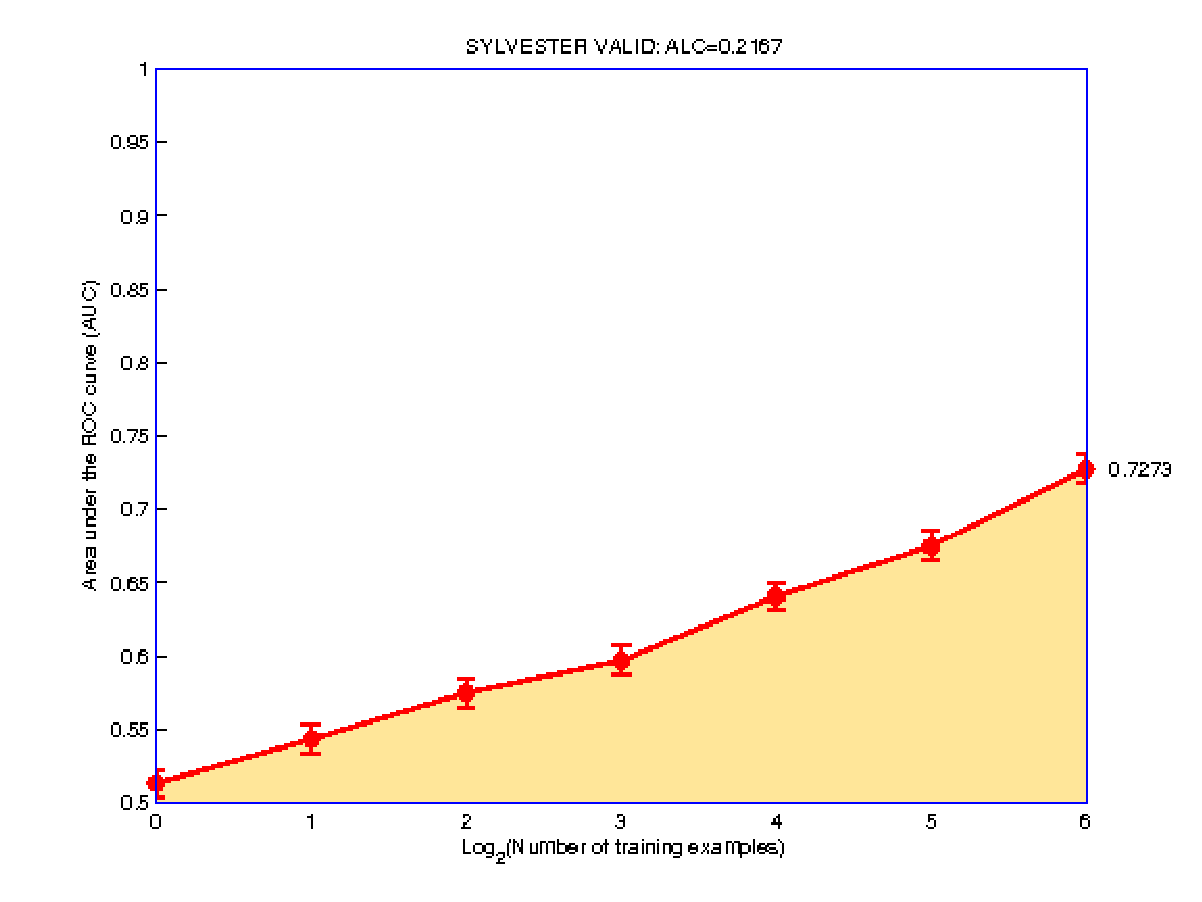
\includegraphics[height=0.15\textheight,keepaspectratio]{article1/images/syl4.pdf}
\caption{Raw Data}
\end{subfigure}
\begin{subfigure}{.3\textwidth}
\centering
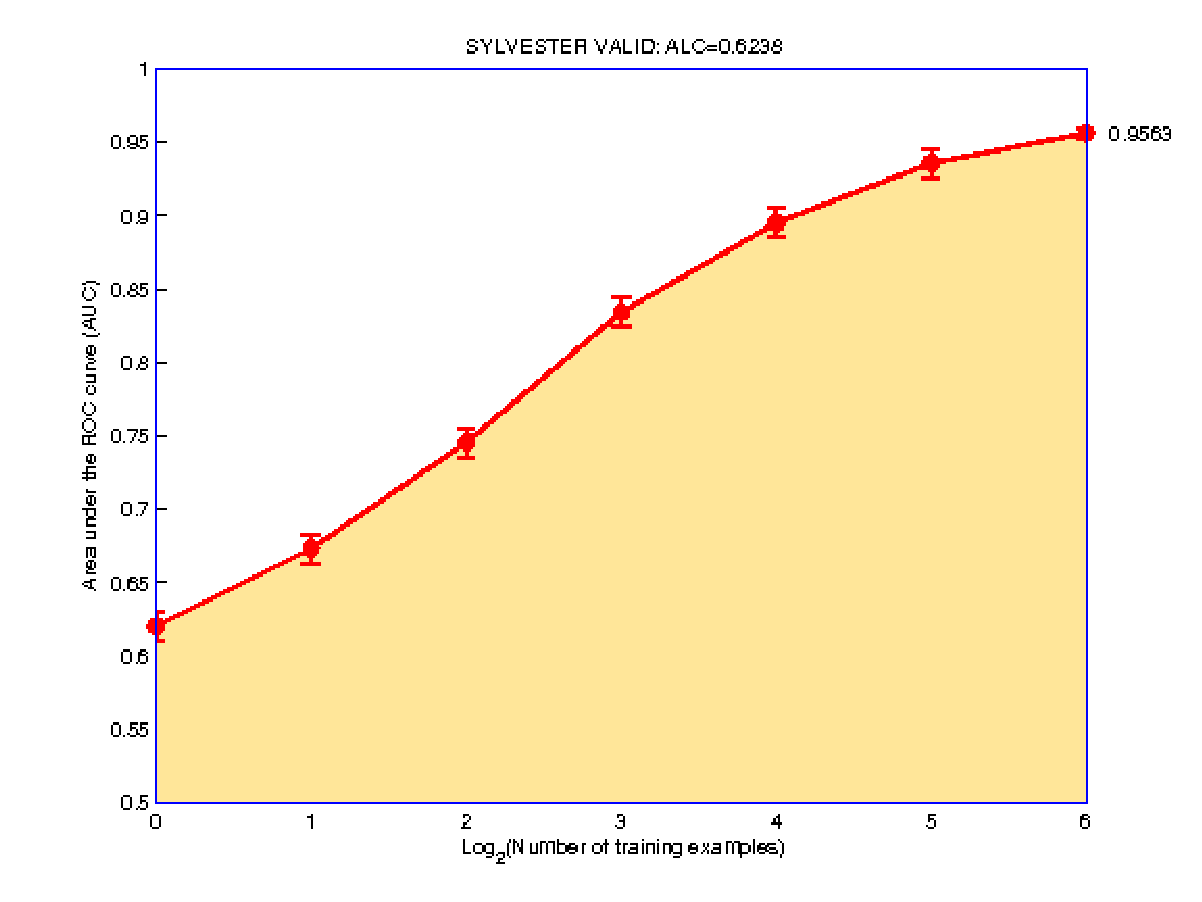
\includegraphics[height=0.15\textheight,keepaspectratio]{article1/images/syl0.pdf}
\caption{1st layer}
\end{subfigure}
\begin{subfigure}{.3\textwidth}
\centering
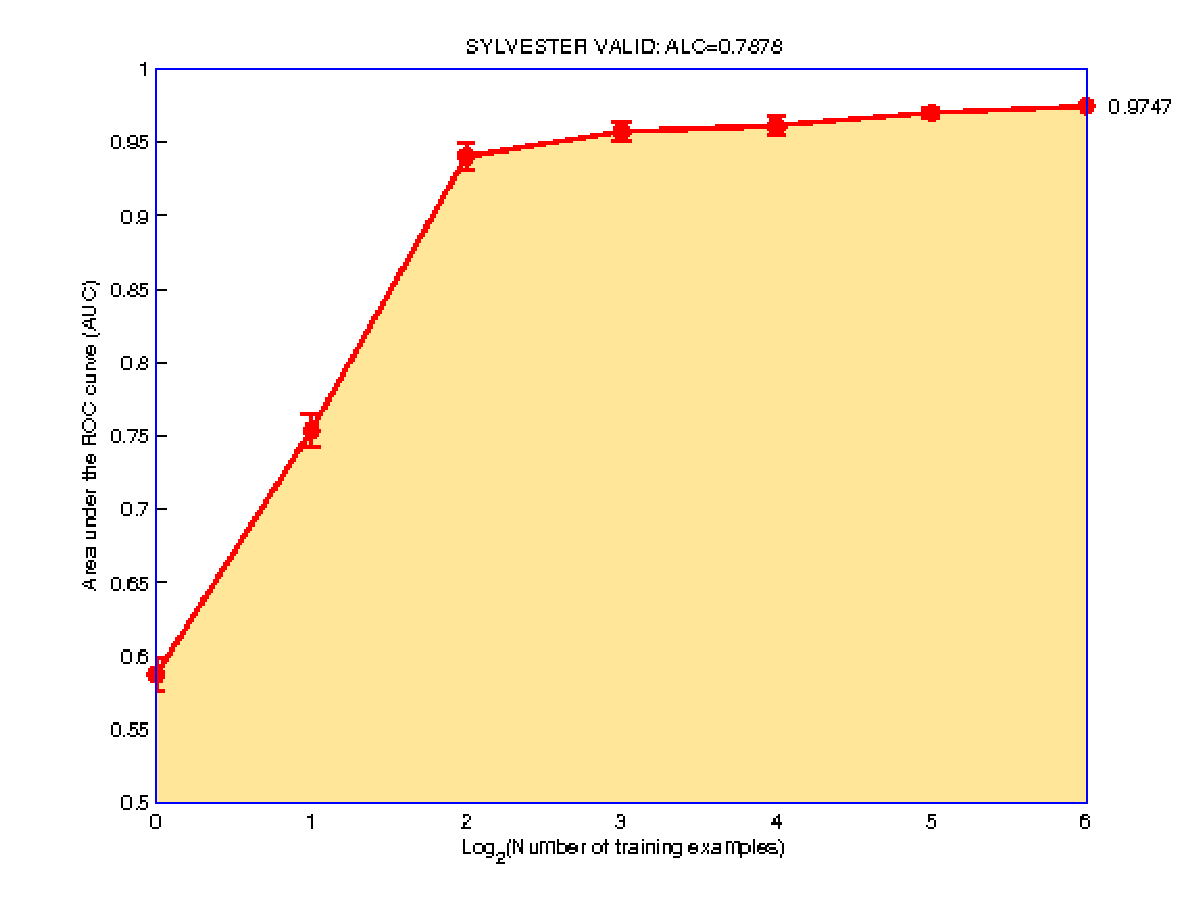
\includegraphics[height=0.15\textheight,keepaspectratio]{article1/images/syl1.pdf}
\caption{2nd layer}
\end{subfigure}\\

\begin{subfigure}{.3\textwidth}
\centering
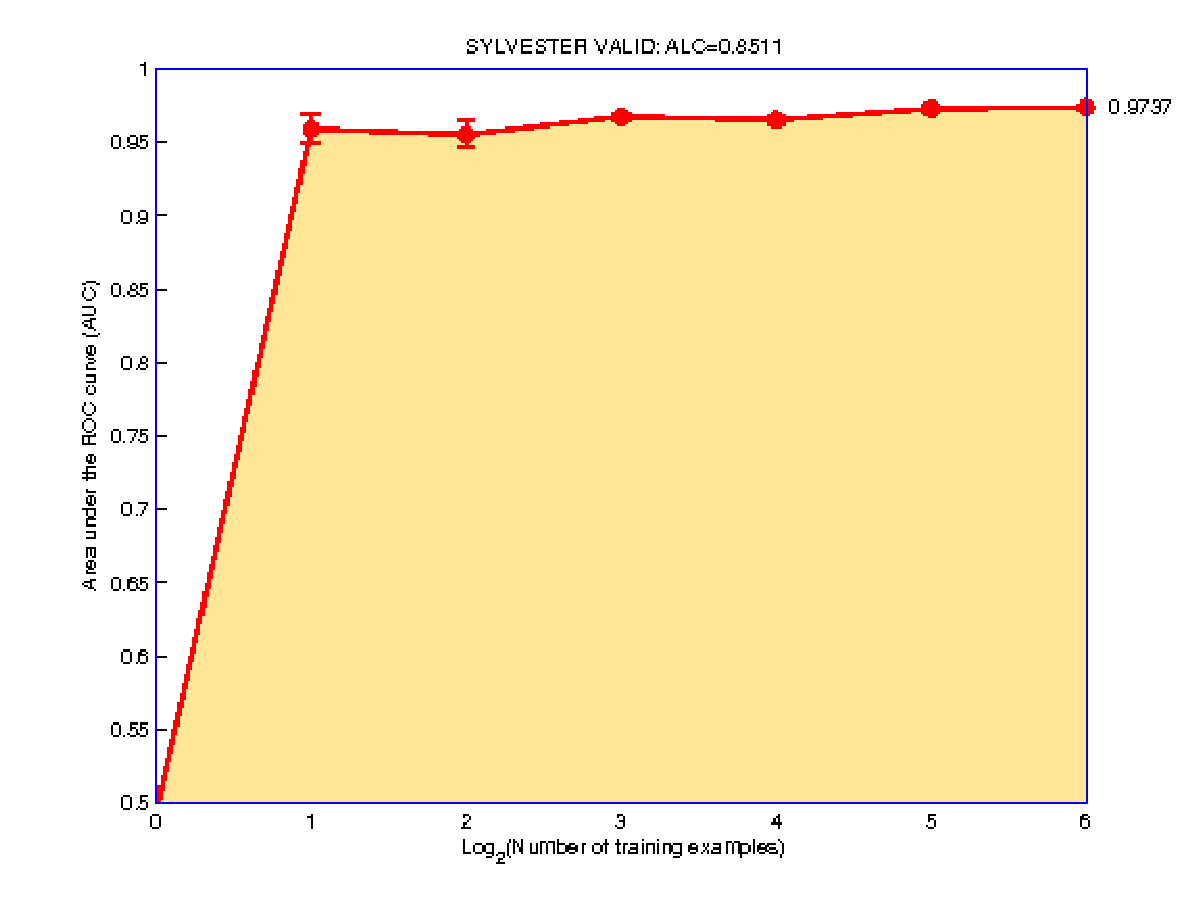
\includegraphics[height=0.15\textheight,keepaspectratio]{article1/images/syl2.pdf}
\caption{3rd layer}
\end{subfigure}
\begin{subfigure}{.3\textwidth}
\centering
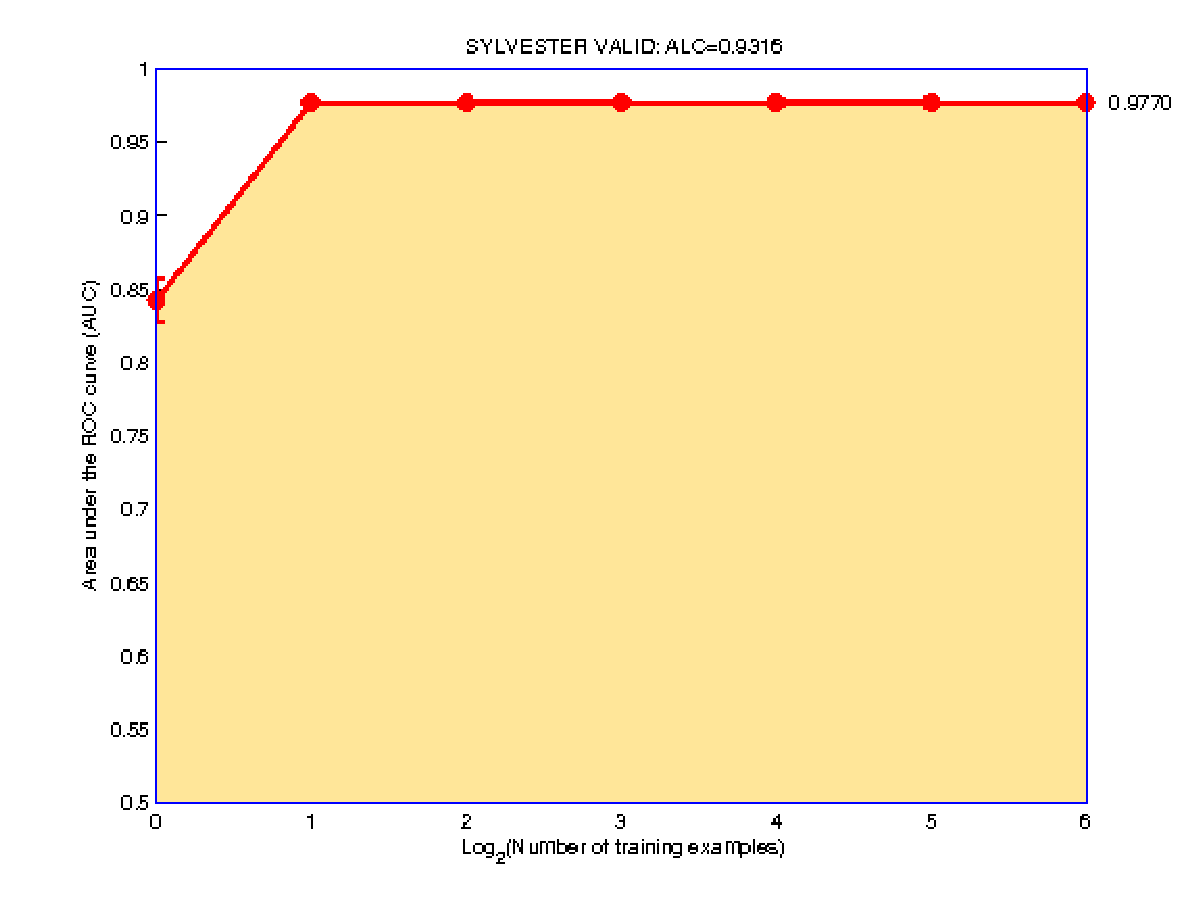
\includegraphics[height=0.15\textheight,keepaspectratio]{article1/images/syl3.pdf}
\caption{t-PCA}
\end{subfigure}
\caption[ALC versus Depth]{Validation performance increases with the depth of our feature
hierarchy for the {\bf SYLVESTER} dataset. ALC: Raw Data ($0.2167$), $1$st
Layer ($0.6238$), $2$nd Layer ($0.7878$), $3$rd Layer ($0.8511$),
t-PCA($0.9316$)}
\label{fig:sylvester}
\end{figure}




Figure \ref{fig:sylvester} shows the evolution of the ALC curve for each layer of the
hierarchy.  Note that at each layer, we only use the top-level features as the
representation.

\paragraph{Results}

This yielded an ALC of $0.85109$ for the validation set and $0.476341$ for the test set.
The difference in ALC may be explained by the fact that Sylvester is the only dataset where
the test set contains more classes than the validation set and, and thus our
assumpptions of equal number of classes might have hurt test performance here.

%\subsubsection{Phase 2}
%We tackled the problem of transduction by creating a better validation criterion. Using the
%criterion described in section \ref{sec:criterion}, we found that a simple Principal
%Component Analysis (PCA) with 8 principal components yielded the best transduction for this
%dataset.

\subsection{RITA}
% EL: The writting style is was really different from the others and it seems
%     the specificity of the u-ssRBM requires more explanation, I leave it to you 
%     Greg to decide whether to rewrite it or not!

% G: Guillaume j'ai tente d'uniformiser ta description avec les autres
% en esperant que ça t'aille


\paragraph{Nature of the data} It corresponds to the CIFAR RGB image dataset and consists of $111,808$ training samples of dimension $7,200$.

\paragraph{Best Architecture}



The $\mu$-ssRBM was initially developed as a model for natural images. As such,
it was a natural fit for the {\bf RITA} dataset. Their ability to learn the pooling
structure was also a clear advantage, since the max-pooling strategy typically
used in vision tasks with convolutional networks~\citep{LeCun98-small} could no longer be employed due to the
obfuscated nature of the dataset.
% The main factors which were considered for
%this series of experiments were: the choice of preprocessing, the
%number of hidden units, the learning rate and number of training epochs,
%the pooling factor $K$ and finally the post-processing.

%Since the likelihood is intractable for large RBMs, one usually relies on a
%proxy (such as classification error) to choose the hyper-parameters. Without
%having access to the labels however, we proceeded as follows.

For pre-processing, each image has been contrast-normalized. Then, we reduced the
dimensionality of the training dataset by learning on the first $1,000$
principal components. For feature extraction, we chose the number of hidden
units to be large enough ($1000$) while still being computationally efficient on GPUs.
The learning rate of $10^{-3}$ and number of training updates ($110,000$
updates with minibatches of size $16$) are chosen such that hidden units have
sparse activations through pools of size $9$, hovering around $10$-$25\%$.
% Finally, we tried $K \in
%\{2,9,50\}$ and uploaded all three representations (after post-processing) to
%the UTLC server. We chose $K=9$ as it gave the best results on the validation
%set.
The post-processing was consistent with the other datasets: we used the
transductive PCA method using only the first $4$ principal components.

\paragraph{Results}

This yielded an ALC score of $0.286$ and $0.437$ for the validation and final
test sets respectively. We also tried to stack $3$ layers of contractive
auto-encoders directly on the raw data and it achieved a valid ALC of
$0.3268$. As it appeared actually transductive, we prefered to keep the
$\mu$-ssRBM in our competition entries because it was trained on the whole
training set.


\section{Conclusion}

The competition setting with different class labels in the validation and the test sets
was quite unusual. The similarity between two classes must be sufficient for
transfer learning to be possible.  %However, similarity is currently assessed
%through human intuition rather than a well defined mathematical property of
%the different classes. 
More formal assessments of class similarity might be useful in such settings.
It is not obvious that the similarity between the
subsets of classes chosen for the different datasets in the context of the
competition is sufficient for an effective generalization, neither that the
similarity between the subsets of classes found in the transfer labels is
representative of the similarity between the classes found in the training, validation
and test datasets.  Finally, for assessing transfer across classes properly
would require a larger number of classes. 
In a future competition, we suggest that both similarity
and representativeness (including number of classes)
should be ensured in a more formal or empirical way.

On all five tasks, we have found the idea of stacking different layer-wise
representation-learning algorithms to work very well. One surprise was the
effectiveness of PCA both as a first layer and a last layer, in a transductive
setting. As core feature-learning blocks, the contractive auto-encoder, the
denoising auto-encoder and spike-and-slab RBM worked best for us on the dense
datasets, while the sparse rectifier denoising auto-encoder worked best on the
sparse datasets.

%\bibliography{strings,ml,aigaion}

\section*{Acknowledgements}

The authors acknowledge the support of the following agencies for research
funding and computing support: NSERC, RQCHP, CIFAR. This is also funded in part by
the French ANR Project ASAP ANR-09-EMER-001.


%{%\small
%\bibliography{strings,ml,aigaion,aaron} %,how_we_won}
%\bibliographystyle{plain}
%\bibliographystyle{natbib}
%}

%\end{document}
